\newcommand{\econtexRoot}{.}
% The \commands below are required to allow sharing of the same base code via Github between TeXLive on a local machine and ShareLaTeX.  This is an ugly solution to the requirement that custom LaTeX packages be accessible, and that ShareLaTeX seems to ignore symbolic links (even if they are relative links to valid locations)
\providecommand{\econtex}{./texmf-local/tex/latex/econtex}
\providecommand{\econtexSetup}{./texmf-local/tex/latex/econtexSetup}
\providecommand{\econtexShortcuts}{./texmf-local/tex/latex/econtexShortcuts}
\providecommand{\econtexBibMake}{./texmf-local/tex/latex/econtexBibMake}
\providecommand{\econtexBibStyle}{./texmf-local/bibtex/bst/econtex}
\providecommand{\notes}{./texmf-local/tex/latex/handout}
\providecommand{\handoutSetup}{./texmf-local/tex/latex/handoutSetup}
\providecommand{\handoutShortcuts}{./texmf-local/tex/latex/handoutShortcuts}
\providecommand{\handoutBibMake}{./texmf-local/tex/latex/handoutBibMake}
\providecommand{\handoutBibStyle}{./texmf-local/bibtex/bst/handout}

  
\documentclass{beamer}
\usepackage{import}
\usepackage{ulem}
\usepackage[Overlays]{optional}
\usepackage{ifthen}
\usepackage{econtexShortcuts}
\usepackage{bbm}
\providecommand{\Ex}{\ensuremath{\mathbb{E}}} % Expectations operator defined in econtex.cls

% if this is uncommented, bullets are shown step by step; comment out to make printable version
\beamerdefaultoverlayspecification{<+->}

% MPCMatch
\provideboolean{MPCMatchVersion}
\setboolean{MPCMatchVersion}{true}
\setboolean{MPCMatchVersion}{false}
\newcommand{\MPCMatch}{\ifthenelse{\boolean{MPCMatchVersion}}}

\newboolean{DiscountSubOn}
\setboolean{DiscountSubOn}{false}
\providecommand{\TimeFactor}{\Discount}
\ifthenelse{\boolean{DiscountSubOn}}{\Discount_{t+1}}{}
\newcommand{\ifTimeSubT}{}
\ifthenelse{\boolean{DiscountSubOn}}{\renewcommand{\ifTimeSubT}{_{T}}}{}
\newcommand{\ifTimeSubNext}{}
\ifthenelse{\boolean{DiscountSubOn}}{\renewcommand{\ifTimeSubNext}{_{t+1}}}{}

\newboolean{RfreeSubOn}
\setboolean{RfreeSubOn}{false}
\providecommand{\R}{\Rfree}
\ifthenelse{\boolean{RfreeSubOn}}{\Rfree_{t+1}}{}

\usepackage{ifthen}
\newboolean{WithOverlays}
\setboolean{WithOverlays}{true}
\usepackage{optional}
\opt{NoOverlays}{\setboolean{WithOverlays}{false}\beamerdefaultoverlayspecification{}}
\usepackage{moreverb}

\usepackage{cancel}
\usepackage{econtexShortcuts}
\usepackage{wasysym}
%\usepackage{dcolumn}
% \usepackage[notocbib]{apacite}
%\renewcommand{\frametitle}{\textbf\frametitle}

% Jirka's definitions
\usepackage[authoryear]{natbib}
\definecolor{jirkasred}{rgb}{0.9,0,0}
\newcommand{\jemph}[1]{{\color{jirkasred}#1}}
\def\newblock{\hskip .11em plus .33em minus .07em}

\mode<presentation>
{
  \usetheme{default}
  % or ...
  \setbeamercovered{transparent}
}

% if this is on, bullets are shown step by step
% \beamerdefaultoverlayspecification{<+->}

%\setbeamertemplate{navigation symbols}{}  % Take away navigation symbols

\usetheme{Frankfurt}

%_____________ Opening slide _______________________

\begin{document}

%\begin{verbatimwrite}{./SolvingMicroDSOPs-Slides-body.tex}

\title[SolvingMicroDSOPs]{\textbf{Structural Estimation of Dynamic Stochastic\\ Optimizing Models of Intertemporal Choice \\ \LARGE{For Dummies!}}}
\author[Carroll]{Christopher Carroll\inst{1}}

\institute{
  \inst{1} Johns Hopkins University and NBER\\   \texttt{ccarroll@jhu.edu} \and
    }
\date{June 2012 \\ {\tiny \url{https://www.econ2.jhu.edu/people/ccarroll/SolvingMicroDSOPs-Slides.pdf}}
}

\begin{frame}[plain]
  \titlepage
\end{frame}

\section{Introduction}

\begin{frame}
\begin{itemize}
\item Efficient Solution Methods for Canonical $C$ problem
\begin{itemize}
\item CRRA utility
\item Plausible (microeconomically calibrated) uncertainty
\item Life cycle or infinite horizon
\end{itemize}
\item How To Add a Second Choice Variable
\item Method of Simulated Moments Estimation of Parameters
\end{itemize}
\end{frame}

\section{The Problem}

\begin{frame}[label=MaxProb]
\frametitle{\large\textbf{The Basic Problem at Date $t$}}

  \begin{equation}\label{eq:MaxProb}
    \max ~ \Ex_{t}\left[ \sum_{n_{\tShkEmp}=0}^{T-t} {\DiscAlt}^{n_{\tShkEmp}} \util({\cLev}_{t+n})\right],
  \end{equation}

\begin{eqnarray}
{\yLev}_{t} & = & {\pLev}_{t}\tShkEmp_{t}
\end{eqnarray}
  \begin{eqnarray}
    \Rfree_{t}   = & \Rfree~\forall~t & \text{- constant interest factor = $1+\rfree$}  \notag
    \\ \pLev_{t+1}  = & \PGro_{t+1}\pLev_{t} &   \text{- permanent labor income dynamics} \label{eq:permincgrow}
    \\ \log ~ \tShkEmp_{t+n} \sim &  ~\mathcal{N}(-\sigma_{\tShkEmp}^{2}/2,\sigma_{\tShkEmp}^{2}) & \text{- lognormal transitory shocks}~\forall~n>0 \notag
                                                                                                    \label{eq:epsdist}
                                                                                                    .
  \end{eqnarray}

\end{frame}

\begin{frame}[label=vrecurse]
\frametitle{\large\textbf{Bellman Equation}}

  \begin{equation}\begin{gathered}\begin{aligned}
    \vLevBF_{t}(\mLev_{t},\pLev_{t})  & = \max_{\cLev_{t}}~ \util(\cLev_{t}) + \Ex_{t}[{\DiscAlt} \vLevBF_{t+1}({\mLev}_{t+1},\pLev_{t+1})]\label{eq:vrecurse}
  \end{aligned}\end{gathered}\end{equation}


\begin{eqnarray*}
   \mLev & - & \text{ `market resources' (net worth plus current income)}
\\ \pLev & - & \text{ permanent labor income }
\end{eqnarray*}

\end{frame}

\section{Tricks}
\subsection{Normalization}
\begin{frame}[label=Normalize]
\frametitle{\large\textbf{Trick: Normalize the Problem}}

  \begin{equation}\begin{gathered}\begin{aligned}
        \null{\vFunc}_{t}({m}_{t})  & = \max_{{c}_{t}} ~~ \uFunc({c}_{t})+
        {\DiscFac}\Ex_{t}[ \PermGroFac_{t+1}^{1-\CRRA}\null{\vFunc}_{t+1}({m}_{t+1})] \label{vtNorm}
        \\         & \text{s.t.} &   \\
        {a}_{t}    & = {m}_{t}-{c}_{t}
        \\      {m}_{t+1}  & = \underbrace{\left(\Rfree/\PermGroFac_{t+1}\right)}_{\equiv \RNrm_{t+1}}{a}_{t}+\TranShkEmp_{t+1} .
      \end{aligned}\end{gathered}\end{equation}


where nonbold variables are bold ones normalized by $\pLev$:
\begin{eqnarray}
\mRat_{t} & = & \mLev_{t}/\pLev_{t}
\end{eqnarray}

Yields $\cFunc_{t}(m)$ from which we can obtain
\begin{eqnarray}
  \cLev_{t}(\mLev_{t},\pLev_{t}) & = & \cFunc_{t}(\mLev_{t}/\pLev_{t})\pLev_{t}
\end{eqnarray}

\end{frame}

\begin{frame}[label=Normalize]
\frametitle{\large\textbf{When Doesn't Normalization Work?}}

\begin{itemize}
\item Non-CRRA utility
\item Non-Friedman (transitory/permanent) income process
\begin{itemize}
\item e.g., AR(1)
\item But micro evidence is consistent with Friedman
\end{itemize}
\end{itemize}

\end{frame}
\subsection{View Problem from End of Period}

\begin{frame}[label=Normalize]
\frametitle{Trick: View Everything from End of Period}

Define 
  \begin{equation}\begin{gathered}\begin{aligned}
        \vEOPt({a}_{t})  & = \Ex_{t}[\DiscFac \PermGroFac_{t+1}^{1-\CRRA}\null{\vFunc}_{t+1}(\RNrm_{t+1} {a}_{t}+{\TranShkEmp}_{t+1})]  \label{eq:vEndtdefn}
      \end{aligned}\end{gathered}\end{equation}

so 
\begin{eqnarray}
  \vFunc_{t}(\mRat_{t}) & = & \max_{\cRat_{t}}~~ \util(\cRat_{t}) + \vEnd_{t}(\mRat_{t}-\cRat_{t})
\end{eqnarray}
with FOC
  \begin{equation}\begin{gathered}\begin{aligned}
        \uFunc^{\prime}({c}_{t})   & = \vEOPt^{\prime}({m}_{t}-{c}_{t}).
        \label{eq:upEqbetaOp}
      \end{aligned}\end{gathered}\end{equation}

and Envelope relation
  \begin{equation}\begin{gathered}\begin{aligned}
        \uFunc^{\prime}({c}_{t})  & = \null{\vFunc}^{\prime}_{t}({m}_{t})\label{eq:Envelope}
      \end{aligned}\end{gathered}\end{equation}


\end{frame}

\subsection{Discretization of Risks}
\begin{frame}[label=DiscretizeFig]
\frametitle{Trick: Discretize the Risks}

E.g.\ use an equiprobable 7-point distribution:\medskip\medskip

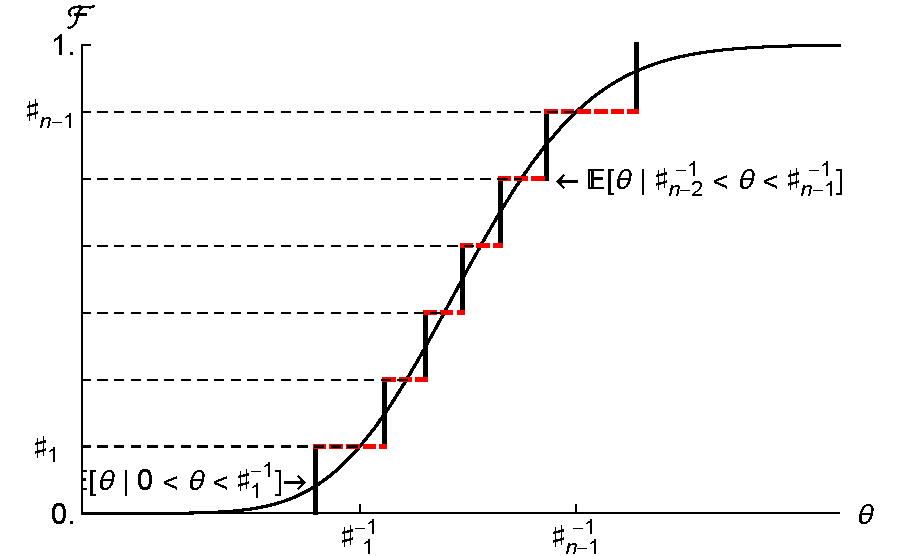
\includegraphics[width=4in]{./Figures/discreteApprox.pdf}

\end{frame}

\begin{frame}[label=DiscretizeEqn]
\frametitle{Trick: Discretize the Risks}

\begin{eqnarray}
        \vEnd_{t}^{\prime}({a}_{t}) & = &  \Discount \Rfree \PGro_{t+1}^{-\CRRA} \left(\frac{1}{n}\right) \sum_{i=1}^{n} \util^{\prime}\left(\cFunc_{t+1}(\Rnorm_{t+1} {a}_{t} + \tShkEmp_{i})\right)
\end{eqnarray}

%\begin{eqnarray}
        \vEnd_{T-1}({a}_{T-1}) & = &   \Discount \PGro_{T}^{1-\CRRA}\left(\frac{1}{n_{\tShkEmp}}\right)\sum_{i=1}^{n_{\tShkEmp}}   \frac{\left( \Rnorm_{T} {a}_{T-1} + \tShkEmp_{i}\right)^{1-\CRRA}}{1-\CRRA} \label{eq:vDiscrete}
\end{eqnarray}


\pause 
So for any particular $\mRat_{T-1}$ the corresponding $\cRat_{T-1}$ can be found
using the FOC:
  \begin{equation}\begin{gathered}\begin{aligned}
        \uFunc^{\prime}({c}_{t})   & = \vEOPt^{\prime}({m}_{t}-{c}_{t}).
        \label{eq:upEqbetaOp}
      \end{aligned}\end{gathered}\end{equation}


\end{frame}
\subsection{Interpolate a Consumption Rule}
\begin{frame}
\frametitle{Trick: Interpolate a Consumption Rule}

\begin{enumerate}
\item Define a grid of points $\vec{\mRat}$ (indexed $\mRat[i]$)
\item Use numerical rootfinder to solve 
$\util^{\prime}(\cRat) = \vEnd^{\prime}_{t}(\mRat[i]-\cRat)$
\begin{itemize}
\item The $\cRat$ that solves this becomes $\cRat[i]$
\end{itemize}
\item Construct interpolating function $\grave{\cFunc}$ by linear interpolation
\begin{itemize}
\item `Connect-the-dots'
\end{itemize}
\end{enumerate}

\end{frame}

\begin{frame}[label=DiscretizeEqn]
\frametitle{Trick: Interpolate a Consumption Rule}

Example: $\vec{\mRat}_{T-1} = \{0.,1.,2.,3.,4.\}$ (solid is `correct' soln)

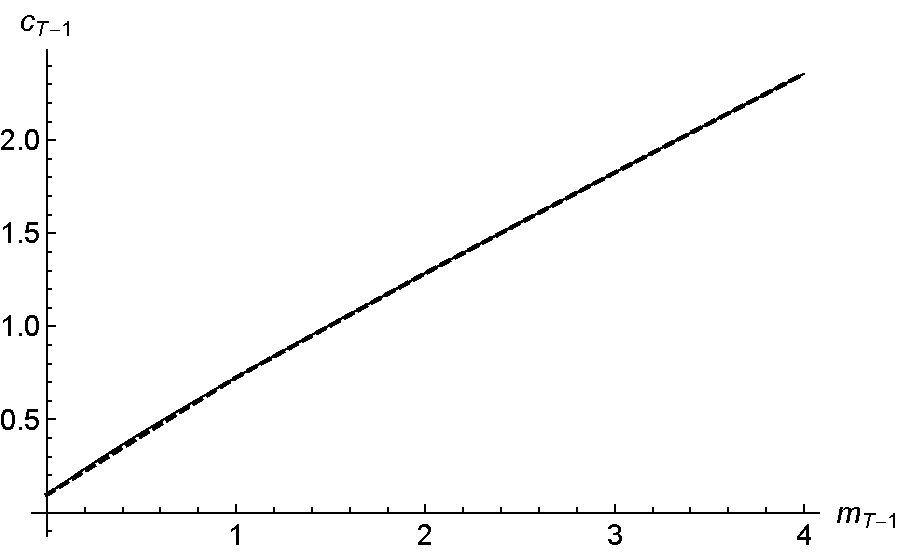
\includegraphics[width=4.0in]{./Figures/PlotcTm1Simple.pdf}

\end{frame}

\begin{frame}[label=vEndtSlow]
\frametitle{Problem: Numerical Rootfinding is {\it Slow}}

Numerical search for values of $\cRat_{T-1}$ satisfying
$\util^{\prime}(\cRat) = \vEnd^{\prime}_{t}(\mRat[i]-\cRat)$ at, say,
6 gridpoints of $\vec{\mRat}_{T-1}$ may require hundreds or even thousands of
evaluations of
\begin{eqnarray}
        \vEnd^{\prime}_{T-1}(\overbrace{{m}_{T-1}-{\cRat}_{T-1}}^{\aRat_{T-1}}) & = &   \Discount_{T} \PGro_{T}^{1-\CRRA}\left(\frac{1}{n}\right)\sum_{i=1}^{n}   \left( \Rnorm_{T} {a}_{T-1} + \tShkEmp_{i}\right)^{-\CRRA} \notag
\end{eqnarray}

\end{frame}

\begin{comment}

\begin{frame}[label=vApprox]
\frametitle{Solution: Approximate $\vEnd$?}

\pause Given $\{\vec{\aRat}_{T-1},\vec{\vEnd}_{T-1}\}$, an approximate function $\grave{\vEnd}_{T-1}$ 
can be constructed by linear interpolation among the points:

\includegraphics[width=4in]{./Figures/PlotOTm1RawVsInt.pdf}

\end{frame}

\begin{frame}
\frametitle{Using $\grave{\vEnd}_{T-1}$ In Optimization}
\begin{eqnarray*}
  \vFunc_{t}(\mRat_{t}) & = & \max_{\cRat_{t}}~~ \util(\cRat_{t}) + \grave{\vEnd}_{t}(\mRat_{t}-\cRat_{t})
\end{eqnarray*}
is {\it much} faster,  but result is bad:
\begin{center}
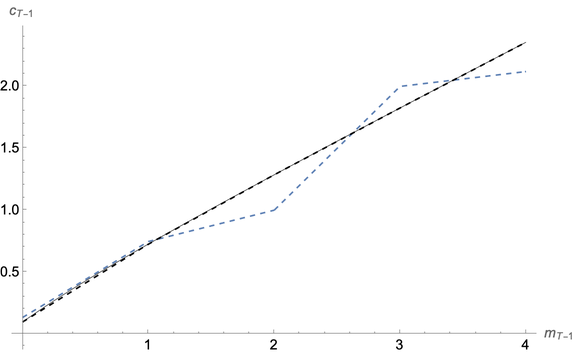
\includegraphics[width=3in]{./Figures/PlotComparecTm1AB}
\end{center}

\end{frame}

\begin{frame}
\frametitle{Approximate $\vEnd_{t}^{\prime}(\aRat)$?}

Better ... but still violates first two principles:
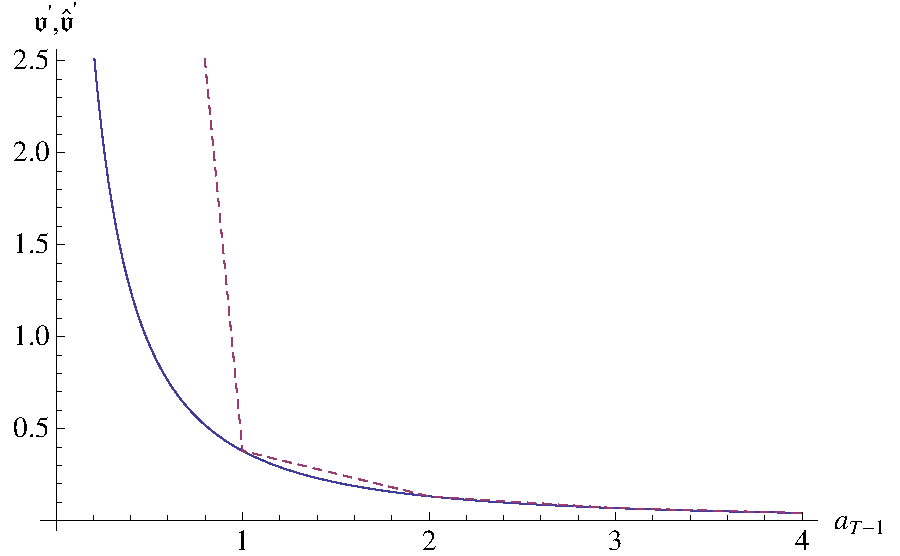
\includegraphics[width=4in]{./Figures/PlotOPRawVSFOC.pdf}

\end{frame}

\end{comment}

\subsection{The Method of Endogenous Gridpoints}
\begin{frame}
\frametitle{Solution: The Method of Endogenous Gridpoints}

\pause 

\begin{itemize}
\item Define vector of {\it end-of-period} asset values $\vec{\aRat}$
\item For each $\aRat[j]$ compute $\vEnd_{t}^{\prime}(\aRat[j])$
\end{itemize}

\pause 

Each of these $\vEnd_{t}^{\prime}[j]$ corresponds to a unique
$\cRat[j]$ via FOC:
\begin{eqnarray}
  \cRat[j]^{-\CRRA} & = & \vEnd_{t}^{\prime}(\aRat[j])
\\ \cRat[j] & = & \left(\vEnd_{t}^{\prime}(\aRat[j])\right)^{-1/\CRRA}
\end{eqnarray}

\pause 

But the DBC says
\begin{eqnarray}
  \aRat_{t} & = & \mRat_{t} - \cRat_{t}
\\ \mRat[j] & = & \aRat[j]+\cRat[j]
\end{eqnarray}

\pause 
So computing $\vEnd_{t}^{\prime}$ at a vector of $\vec{\aRat}$ values has produced for us the corresponding $\vec{\cRat}$ and $\vec{\mRat}$ 
values at virtually no cost!  

\pause 
\medskip 
From these we can interpolate as before to construct $\grave{\cFunc}_{t}(\mRat)$.

\end{frame}

\begin{frame}
\frametitle{Why Directly Approximating $\vFunc_{t}$ is a Bad Idea}

Principles of Approximation

\begin{itemize}
\item Hard to approximate things that approach $\infty$ for relevant $\mRat$
\begin{itemize}
\item Not a prob for Rep Agent models: `relevant' $\mRat$'s are $\approx$ SS
\end{itemize}
\item Hard to approximate things that are highly nonlinear 
%\item Best to approximate things that directly govern behavior
\end{itemize}

\end{frame}

\begin{frame}
\frametitle{Approximate Something That Would Be Linear in PF Case}

\medskip

Perfect Foresight Theory:
\begin{eqnarray}
  \cFunc_{t}(\mRat) & = & (\mRat+\hEnd_{t})\MinMPC_{t} 
\end{eqnarray}
for market resources $\mRat$ and end-of-period human wealth $\hEnd$.

\medskip\medskip
\pause 

This is why it's a good idea to approximate $\cFunc_{t}$ 

\pause \medskip\medskip

Bonus: Easy to debug programs by setting $\sigma^{2} = 0$ and
testing whether numerical solution matches analytical!

\end{frame}

\subsection{Approximate Inverted Functions}
\begin{frame}%[ValFnApprox]
\frametitle{But What if You {\it Need} the Value Function?}

Perfect foresight value function:
  \begin{equation}\begin{gathered}\begin{aligned}
    \bar{\vFunc}_{t}({m}_{t})  & = \util(\bar{\cRat}_{t})\mathbb{C}_{t}^{T}\label{eq:vFuncPF}
    \\  & = \util(\bar{c}_{t}) \MinMPC_{t}^{-1} % 20190820
    \\  & = \util((\aboveMin \mRat_{t}+\aboveMin \hEnd_{t})\MinMPC_{t}) \MinMPC_{t}^{-1} % 20190820
    \\  & = \util(\aboveMin \mRat_{t}+\aboveMin \hEnd_{t})\MinMPC_{t}^{1-\CRRA} \MinMPC_{t}^{-1} % 20190820
    \\  & = \util(\aboveMin \mRat_{t}+\aboveMin \hEnd_{t})\MinMPC_{t}^{-\CRRA}  % 20190820
  \end{aligned}\end{gathered}\end{equation}
  where the second line uses the fact demonstrated in \cite{BufferStockTheory} that $\mathbb{C}_{t}=\MPC^{-1}_{t}$. % 20190820

  This can be transformed as
  \begin{equation*}\begin{gathered}\begin{aligned}
    \bar{\vInv}_{t}  & \equiv  \left((1-\CRRA)\bar{\vFunc}_{t}\right)^{1/(1-\CRRA)}
    \\  & = \cRat_{t}(\mathbb{C}_{t}^{T})^{1/(1-\CRRA)}
    \\  & = (\aboveMin \mRat_{t}+\aboveMin \hEnd_{t})\MinMPC_{t}^{-\CRRA/(1-\CRRA)}   % 20190820
  \end{aligned}\end{gathered}\end{equation*}

which is linear.  

\medskip\medskip
\pause If you need the value function, approximate the {\it inverted} value function to generate $\grave{\vInv}_{t}$ 
and then obtain your approximation from 
\begin{eqnarray}
  \grave{\vFunc}_{t} & = & \util(\grave{\vInv}_{t})
\end{eqnarray}

\end{frame}

\subsection{Derivatives}
\begin{frame}
\frametitle{Approximate Slope Too}

\cite{BufferStockTheory} shows that $\cFunc^{\mRat}_{t}$ exists everywhere.
\medskip

\pause 
Define {\it consumed} function and its derivative as 
\begin{eqnarray}
  \cEndFunc_{t}(\aRat) & = & (\vEnd^{\prime}_{t}(\aRat))^{-1/\CRRA}
\\ \cEndFunc_{t}^{\aRat}(\aRat) & = & -(1/\CRRA)\left(\vEnd_{t}^{\prime}({a})\right)^{-1-1/\CRRA} \vEnd_{t}^{\prime\prime}(\aRat) 
\end{eqnarray}

\pause 
and using chain rule it is easy to show that
\begin{eqnarray}
 \cFunc^{\mRat}_{t} & = & \cEndFunc^{\aRat}_{t}/(1+\cEndFunc^{\aRat}_{t})
\end{eqnarray}

\end{frame}

\begin{frame}
\frametitle{To Implement: Modify Prior Procedures in Two Ways}
\begin{enumerate}
\item Construct $\vec{\cFunc}^{\mRat}_{t}$ along with $\vec{\cFunc}_{t}$ in EGM algorithm
\item Approximate $\cFunc_{t}(m)$ using piecewise Hermite polynomial
\begin{itemize}
\item Exact match to both level and derivative at set of points
\end{itemize}
\end{enumerate}
\end{frame}

\subsection{Improving the $\aRat$ Grid}

\begin{frame}
\frametitle{Problem: $\Alt{\cFunc}$ Below Bottom $\mRat$ Gridpoint and Extrapolation}

Consider what happens as ${a}_{T-1}$ approaches $\underline{a}_{T-1}\equiv-\underline{\tShkEmp}\Rnorm_{T}^{-1}$,
\begin{eqnarray*}
        \lim_{{\aRat} \downarrow \underline{a}_{T-1}} \vEnd_{T-1}^{\prime}({\aRat}) & = &
        \lim_{{\aRat} \downarrow \underline{a}_{T-1}} \Discount \Rfree \PGro_{T}^{-\CRRA} \left(\frac{1}{n}\right) \sum_{i=1}^{n} \left( {\aRat} \Rnorm_{T}+ \tShkEmp_{i}\right)^{-\CRRA}
\\ & = & \infty
\end{eqnarray*}

This means our lowest value in $\vec{\aRat}_{T-1}$ should be $> \underline{\aRat}_{T-1}$.  

\medskip
Suppose we construct $\Alt{\cFunc}$ by linear interpolation:
\begin{eqnarray*}
  \Alt{\cFunc}_{T-1}(\mRat) &  = & \Alt{\cFunc}_{T-1}(\vec{\mRat}_{T-1}[1])+\Alt{\cFunc}_{T-1}^{\prime}(\vec{\mRat}_{T-1}[1])({\mRat}-\vec{\mRat}_{T-1}[1]) \label{eq:ExtrapLin}
\end{eqnarray*}

True $\cFunc$ is strictly concave 
$\Rightarrow \exists \mRat^{-} > \underline{\mRat}_{T-1}$  for which $\mRat^{-}-\Alt{\cFunc}_{T-1}(\mRat^{-}) < \underline{\aRat}_{T-1}$

\end{frame}

\begin{frame}
\frametitle{Solution: Hard-Code the Bottom Point}

Theory says that
\begin{eqnarray}
  \lim_{\mRat \downarrow \underline{\mRat}_{T-1}} \cFunc_{T-1}(\mRat) & = & 0
\\ \lim_{\mRat \downarrow \underline{\mRat}_{T-1}} \cFunc_{T-1}^{\mRat}(\mRat) & = & \MaxMPC_{T-1}
\end{eqnarray}

\medskip 

\begin{enumerate}
\item Redefine $\vec{\aRat}$ {\it relative} to $\uline{\aRat}_{T-1}$
\item Construct corresponding $\vec{\mRat}_{T-1}$ and $\vec{\cRat}_{T-1}$
\item Prepend $\uline{\mRat}_{T-1}$ to $\vec{\mRat}_{T-1}$
\item Prepend $0.$ to $\vec{\cRat}_{T-1}$
\item Prepend $\MaxMPC_{T-1}$ to $\vec{\MPC}_{T-1}$
\end{enumerate}
then proceed as before.

\end{frame}

\begin{frame}
\frametitle{Trick: Improving the $\aRat$ Grid}
Grid Spacing: Uniform

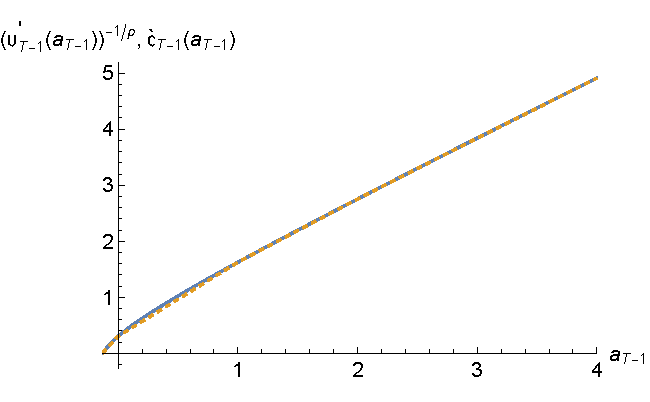
\includegraphics[width=4in]{./Figures/GothVInvVSGothC.pdf}

\end{frame}

\begin{frame}
\frametitle{Trick: Improving the $\aRat$ Grid}
Grid Spacing: Same $\{\uline{\aRat},\bar{\aRat}\}$ But Triple Exponential $e^{e^{e^{...}}}$ Growth

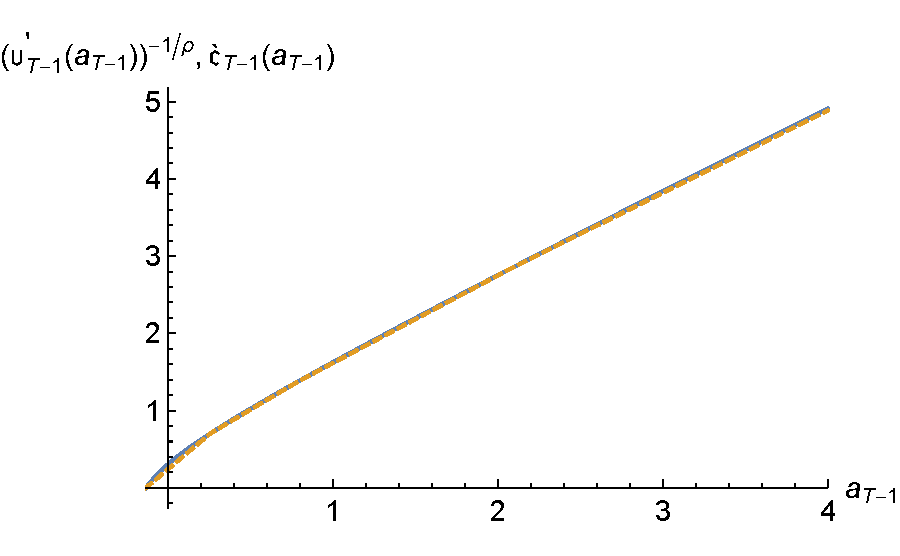
\includegraphics[width=4in]{./Figures/GothVInvVSGothCEEE.pdf}

\end{frame}

\subsection{The Method of Moderation}

\begin{frame}[label=MoM]
\frametitle{The Method of Moderation}

\begin{itemize}
\item Further improves speed and accuracy of solution
\item See my talk at the conference!
\end{itemize}

\end{frame}

\begin{frame}
\frametitle{Imposing `Artificial' Borrowing Constraints}
\begin{eqnarray*}
{\vFunc}_{T-1}({m}_{T-1}) & = & \max_{\cRat_{T-1}} ~~ \util({c}_{T-1}) + \Ex_{T-1} [\Discount \PGro_{T}^{1-\CRRA}{\vFunc}_{T}({m}_{T})] \label{eq:ConstrArt}
\\ & \mbox{s.t.}&   
\\ {a}_{T-1} & = & {m}_{T-1} - {c}_{T-1}
\\ {m}_{T} & = & \Rnorm_{T} {a}_{T-1} + \tShkEmp_{T}
\\ {a}_{T-1} & \geq & 0 .
\end{eqnarray*}


\pause 

Define $\grave{\cFunc}^{*}_{t}$ as soln to unconstrained problem.  Then
\begin{eqnarray}
        \grave{\cFunc}_{T-1}({m}_{T-1}) & = & \min[{m}_{T-1},\grave{\cFunc}^{\ast}_{T-1}({m}_{T-1})] \label{eq:LiqCons}.
\end{eqnarray}


\end{frame}

\begin{frame}
\frametitle{Imposing `Artificial' Borrowing Constraints}

Point where constraint makes transition from binding to not is
\begin{eqnarray*}
    \util^{\prime}(\mRat_{T-1}^{\#}) & = & \vEnd^{\prime}_{T-1}(0.)
\\  \mRat_{T-1}^{\#} & = & \left(\vEnd^{\prime}_{T-1}(0.)\right)^{-1/\CRRA}
\end{eqnarray*}
\pause\medskip

Procedure is very easy:
\begin{itemize}
\item Add $0.$ as first point in $\vec{\aRat}$
\item $\Rightarrow \vec{\mRat}[1] = \mRat_{T-1}^{\#}$
\item Above $\mRat_{T-1}^{\#}$, $\grave{\cFunc}_{T-1}(\mRat)$ obtained as before
\item Below $\mRat_{T-1}^{\#}$, $\grave{\cFunc}_{T-1}(\mRat)=\mRat$
\end{itemize}

\end{frame}

\begin{frame}
\frametitle{Imposing `Artificial' Borrowing Constraints}
\begin{figure}
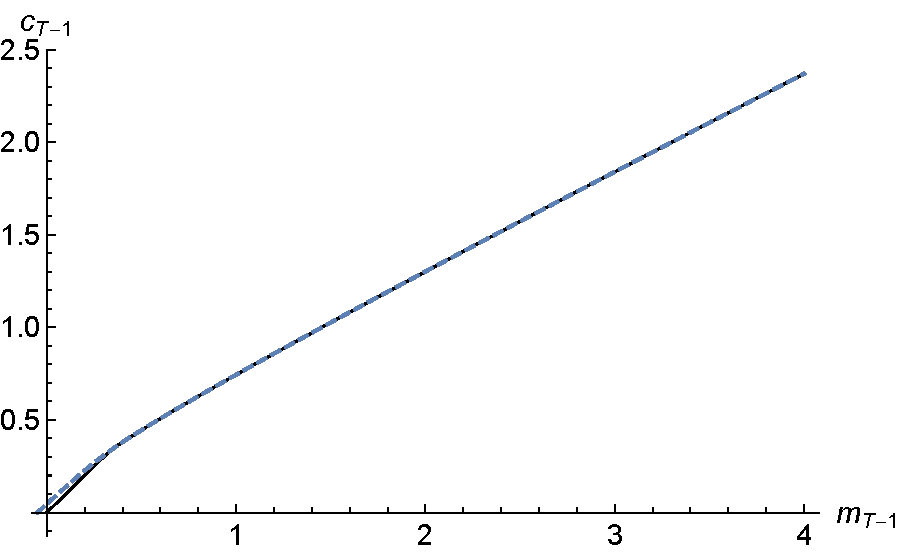
\includegraphics[width=4in]{./Figures/cVScCon.pdf}
        \caption{Constrained (solid) and Unconstrained (dashed) Consumption}
        \label{fig:cVScCon}
\end{figure}

\end{frame}

\begin{frame}%[Recursion]
\frametitle{Recursion: Period $t$ Solution Given Period $t+1$}
\begin{enumerate}
\item Construct 
\begin{eqnarray}
        \cEndFunc_{t,i} & = & \left(\vEnd_{t}^{\prime}({a}_{t,i})\right)^{-1/\CRRA},
\\                            & = & \left(\Discount \Ex_{t} \left[\Rfree \PGro_{t+1}^{-\CRRA}(\grave{\cFunc}_{t+1}(\Rnorm_{t+1} {a}_{t,i} +      {\tShkEmp}_{t+1}))^{-\CRRA}\right]\right)^{-1/\CRRA}, \label{eq:vEndeq}
\MPCMatch{\\        \cEndFunc^{a}_{t,i} & = & -(1/\CRRA)\left(\vEnd_{t}^{\prime}({a}_{t,i})\right)^{-1-1/\CRRA} \vEnd_{t}^{\prime\prime}(\aRat_{t,i}),}{}
\end{eqnarray}

\item Call the result $\vec{\cRat}_{t}$ and generate the corresponding $\vec{\mRat}_{t}=\vec{\cRat}_{t}+\vec{\aRat}_{t}$
\item Interpolate to create $\grave{\cRat}_{t}(\mRat)$
\end{enumerate}

\end{frame}

\begin{frame}%[Convergence]
\frametitle{Consumption Rules $\grave{\cFunc}_{T-n}$ Converge}

\begin{figure}
        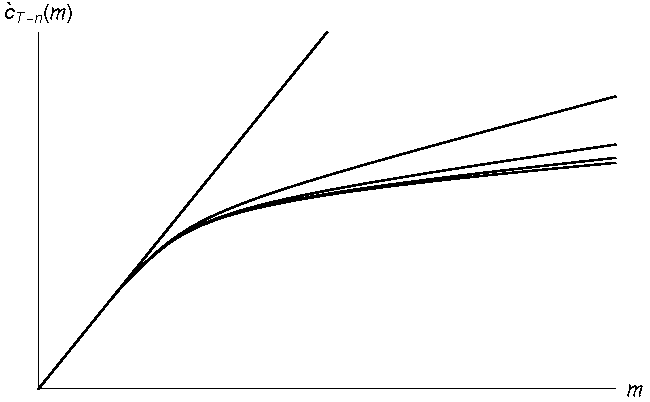
\includegraphics[width=4in]{./Figures/PlotCFuncsConverge.pdf}
        \caption{Converging $\grave{\cFunc}_{T-n}({\mRat})$ Functions for $n=\{1,5,10,15,20\}$}
        \label{fig:PlotCFuncsConverge}
\end{figure}

\end{frame}

\section{Multiple Control Variables}
\begin{frame}
\frametitle{Portfolio Choice}

Now the consumer has a choice between a risky and a safe asset.  \pause The portfolio
return is
  \begin{eqnarray}
    \Rport_{t+1} & = & \Rfree(1-\varsigma_{t}) + \Risky_{t+1}\varsigma_{t} \label{eq:return1}
    \\              & = & \Rfree + (\Risky_{t+1}-\Rfree) \varsigma_{t} \label{eq:return2}
  \end{eqnarray}

\pause so (setting $\PGro=1$) the maximization problem is \pause 
  \begin{equation*}\begin{gathered}\begin{aligned}
    {\vFunc}_{t}({m}_{t})  & = \max_{\{{c}_{t},\varsigma_{t}\}}   ~~ \util({c}_{t}) +  \Discount
                                \Ex_{t}[{\vFunc}_{t+1}({m}_{t+1})]
    \\      & \text{s.t.} &
    \\      \Rport_{t+1}  & = \Rfree + (\Risky_{t+1}-\Rfree) \varsigma_{t}
    \\      {m}_{t+1}  & = ({m}_{t}-{c}_{t})\Rport_{t+1} + \tShkEmp_{t+1}
    \\  0       \leq & \varsigma_{t} & \leq 1, \label{eq:noshorts}
  \end{aligned}\end{gathered}\end{equation*}


\end{frame}

\begin{frame}
\frametitle{Portfolio Choice}

The FOC with respect to $\cRat_{t}$ now yields an Euler equation
  \begin{equation}\begin{gathered}\begin{aligned}
        \uFunc^{{c}}({c}_{t})  & = \Ex_{t}[\DiscFac {\Rport}_{t+1} \uFunc^{{c}}({c}_{t+1})]. \label{eq:EulercRiskyR}
      \end{aligned}\end{gathered}\end{equation}

\pause
while the FOC with respect to the portfolio share yields
  \begin{equation}\begin{gathered}\begin{aligned}
    0  & = \Ex_{t}[{\vFunc}_{t+1}^{\prime}({m}_{t+1})(\Risky_{t+1}-\Rfree){a}_{t}]
    \\         & = {a}_{t}\Ex_{t}\left[\util^{\prime}\left(\cFunc_{t+1}({m}_{t+1})\right)(\Risky_{t+1}-\Rfree)\right] \label{eq:FOCw}.
  \end{aligned}\end{gathered}\end{equation}


\end{frame}

\section{The Infinite Horizon}
\subsection{Convergence}
\begin{frame}
\frametitle{Convergence}

When the problem satisfies certain conditions~(\cite{BufferStockTheory}),
it defines a `converged' consumption rule with a `target' ratio $\check{\mRat}$
that satisfies:
\begin{eqnarray}
  \Ex_{t}[\mRat_{t+1}/\mRat_{t}] & = & 1 \text{~if $\mRat_{t} = \check{\mRat}$}
\end{eqnarray}

\pause 

Define the target $\mRat$ implied by the consumption rule $\cFunc_{t}$ as $\check{\mRat}_{t}$.

\medskip\pause
Then a plausible metric for convergence is to define some value $\epsilon$ and to declare
the solution to have converged when
\begin{eqnarray}
  |\check{\mRat}_{t+1}-\check{\mRat}_{t}| & < & \epsilon
\end{eqnarray}

\end{frame}

\subsection{Tricks}
\begin{frame}
\frametitle{Trick: Coarse then Fine $\tShkEmp$}

\begin{enumerate}
\item Start with coarse grid for $\tShkEmp$ (say, 3 points)
\item Solve to convergence; call period of convergence $n$
\item Construct finer grid for $\tShkEmp$ (say, 7 points)
\item Solve for period $T-n-1$ assuming $\Alt{\cFunc}_{T-n}$ 
\item Continue to convergence
\end{enumerate}

\end{frame}

\begin{frame}
\frametitle{Trick: Coarse then Fine $\vec{\aRat}_{T-1}$}

\begin{enumerate}
\item Start with coarse grid for $\vec{\aRat}$ (say, 5 gridpoints)
\item Solve to convergence; call period of convergence $n$
\item Construct finer grid for $\vec{\aRat}$ (say, 20 points)
\item Solve for period $T-n-1$ assuming $\Alt{\cFunc}_{T-n}$ 
\item Continue to convergence
\end{enumerate}

\end{frame}

\section{Structural Estimation}
\subsection{Life Cycle Model}

\begin{frame}
\frametitle{Life Cycle Maximization Problem}
\begin{eqnarray*}
    {\vFunc}_{t}({m}_{t}) & = & \max_{{c}_{t}} \left\{\util({c}_{t})+\beth\Alive_{t+1}\hat{\Discount}_{t+1}
    \Ex_{t}[(\pShk_{t+1}\PGro_{t+1})^{1-\CRRA}{\vFunc}_{t+1}({m}_{t+1})] \right\}   \\
         & \text{s.t.} &   \nonumber \\
    {a}_{t}   & = & {m}_{t}-{c}_{t} \nonumber
\\      {m}_{t+1} & = & {a}_{t}\underbrace{\left(\frac{\Rfree}{\pShk_{t+1}\PGro_{t+1}}\right)}_{\equiv \Rnorm_{t+1}}+\tShkEmp_{t+1}
\end{eqnarray*}

    \begin{eqnarray*}
      \Alive _{s} &:&\text{probability alive (not dead) until age $s$ given alive at age $s-1$}
      \\      {\hat{\Discount}}_{s} &:&\text{time-varying discount factor between age $s-1$ and $s$}
      \\     \Psi_{s} &:&\text{mean-one shock to permanent income}
      \\     \beth &:&\text{time-invariant discount factor}
    \end{eqnarray*}
  

\end{frame}

\begin{frame}
\frametitle{Details follow~\cite{cagettiWprofiles}}
\begin{itemize}
\item Parameterization of Uncertainty
\item Probability of Death
\item Demographic Adjustments to $\Discount$
\end{itemize}
\end{frame}

\begin{frame}
\frametitle{Empirical Wealth Profiles}
\begin{figure}
    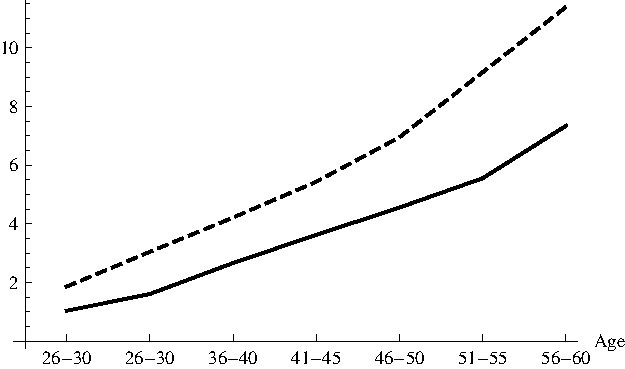
\includegraphics[width=3.5in]{./Figures/PlotMeanMedianSCFcollegeGrads.pdf}
    \caption{$\mRat$ from SCF (means (dashed) and medians (solid))}
    \label{fig:MeanMedianSCF}
\end{figure}
\end{frame}

\begin{frame}
\frametitle{Simulated Moments}

Given a set of parameter values $\{\CRRA,\beth\}$:
\begin{itemize}
\item Start at age 25 with empirical $\mRat$ data
\item Draw shocks using calibrated $\sigma^{2}_{\pShk}$,$\sigma^{2}_{\tShkEmp}$
\item Consume according to solved $\cFunc_{t}$
\end{itemize}
\pause 
$\Rightarrow \mRat$ distribution by age
\end{frame}

\begin{frame}
\frametitle{Choose What to Simulate}
  \begin{equation}\begin{gathered}\begin{aligned}
        \lefteqn{    \texttt{GapEmpiricalSimulatedMedians$[\CRRA,\beth]$:=}}    \nonumber \\
        &[&\texttt{ConstructcFuncLife$[\CRRA,\beth]$;}\nonumber\\
        &\texttt{Simulate;}\nonumber\\
        &\sum\limits_{i}^{N}\weight _{i}\left|\varsigma_{i}^{\tau }-\mathbf{s}^{\tau}(\xi )\right| \nonumber\\
        &];&\nonumber
      \end{aligned}\end{gathered}\end{equation}

\end{frame}

\begin{frame}
\frametitle{Calculate Match Between Theory and Data}
\begin{eqnarray}
\xi & = & \{\CRRA,\beth\}
\end{eqnarray}
solve
\begin{equation}
    \min_{\xi}\sum\limits_{i}^{N}\weight _{i}\left|\varsigma_{i}^{\tau }-\mathbf{s}^{\tau}(\xi )\right|\label{eq:StructEstim}
\end{equation}


\end{frame}
\begin{frame}
\frametitle{Bootstrap Standard Errors (\cite{horowitzBootstrap})}

Yields estimates of 
    \begin{table}[h]
      \caption{Estimation Results}\label{tab:EstResults}
      \center
      \begin{tabular}{cc}
        \hline
        $\CRRA $ & ${\beth}$\\
        \hline
        $4.68$ & $1.00$\\
        $(0.13)$ & $(0.00)$\\
        \hline
      \end{tabular}
    \end{table}
  


\end{frame}

\begin{frame}
\frametitle{Contour Plot}
\begin{figure}
     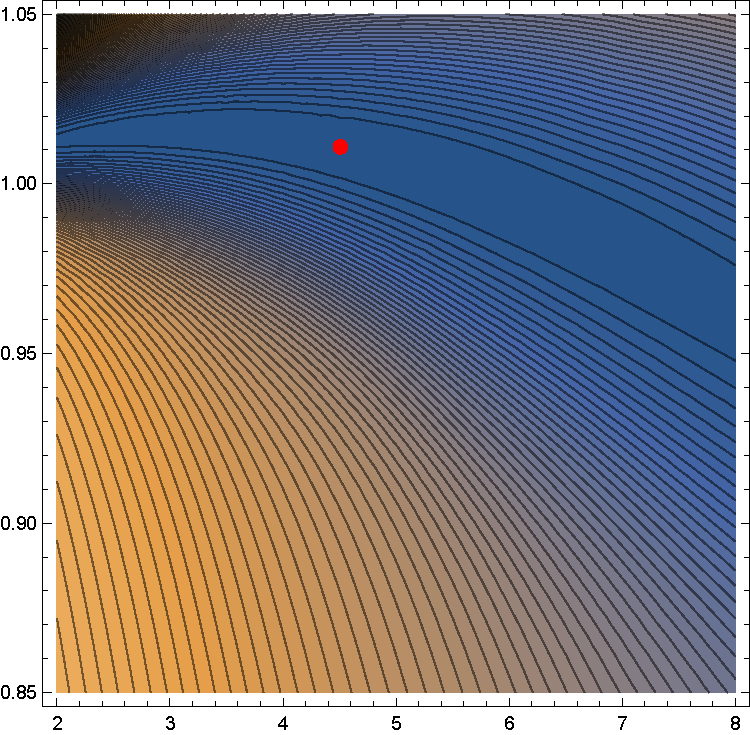
\includegraphics[width=2.5in]{./Figures/PlotContourMedianStrEst.pdf}
    \caption{Point Estimate and Height of Minimized Function}
    \label{fig:PlotContourMedianStrEst}
\end{figure}

\end{frame}

\beamerdefaultoverlayspecification{<*>}

\begin{frame}[allowframebreaks]
\frametitle{\textbf{References}}
\tiny
\input handoutBibMake
\end{frame}

\end{document}
